\documentclass[border=4pt]{standalone}

\usepackage{amsmath}
\usepackage{tikz}
\usepackage{mathdots}
\usepackage{yhmath}
\usepackage{cancel}
\usepackage{color}
\usepackage{siunitx}
\usepackage{array}
\usepackage{multirow}
\usepackage{amssymb}
\usepackage{gensymb}
\usepackage{tabularx}
\usepackage{booktabs}
\usetikzlibrary{fadings}
\usetikzlibrary{patterns}


\begin{document}
 




\tikzset{every picture/.style={line width=0.75pt}} %set default line width to 0.75pt        

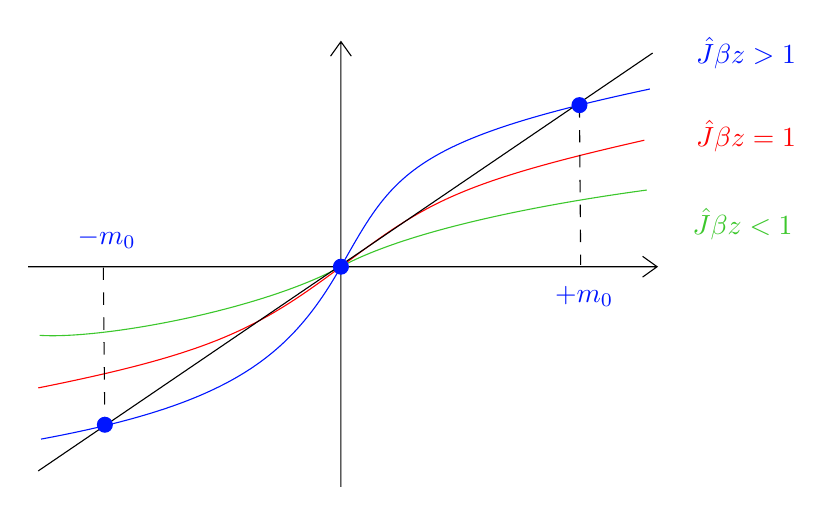
\begin{tikzpicture}[x=0.75pt,y=0.75pt,yscale=-1,xscale=1]
%uncomment if require: \path (0,619); %set diagram left start at 0, and has height of 619

%Shape: Axis 2D [id:dp6363211858926949] 
\draw  (175.5,208.44) -- (478.5,208.44)(326.15,100) -- (326.15,314.5) (471.5,203.44) -- (478.5,208.44) -- (471.5,213.44) (321.15,107) -- (326.15,100) -- (331.15,107)  ;
%Curve Lines [id:da6525211977239838] 
\draw [color={rgb, 255:red, 60; green, 199; blue, 44 }  ,draw opacity=1 ]   (181,241.5) .. controls (211,243.5) and (287.09,229.5) .. (326.15,208.44) .. controls (365.21,187.37) and (444,175.5) .. (473.5,171.5) ;


%Curve Lines [id:da8493047512827328] 
\draw [color={rgb, 255:red, 255; green, 3; blue, 3 }  ,draw opacity=1 ]   (180.33,266.83) .. controls (263.67,250.17) and (286.15,238.44) .. (326.15,208.44) .. controls (366.15,178.44) and (381,168.17) .. (472.33,147.5) ;


%Curve Lines [id:da3038005801224477] 
\draw [color={rgb, 255:red, 0; green, 21; blue, 255 }  ,draw opacity=1 ]   (181.67,291.5) .. controls (271.67,274.83) and (301,252.83) .. (326.15,208.44) .. controls (351.3,164.04) and (359,147.5) .. (475,122.83) ;


%Straight Lines [id:da49427458124243695] 
\draw    (180.33,306.83) -- (476.33,105.5) ;


%Straight Lines [id:da05546458007676791] 
\draw  [dash pattern={on 4.5pt off 4.5pt}]  (211.67,208.83) -- (212.42,284.58) ;


%Straight Lines [id:da04556535029655029] 
\draw  [dash pattern={on 4.5pt off 4.5pt}]  (441.08,130.58) -- (441.67,207.5) ;


%Shape: Circle [id:dp799330245440671] 
\draw  [color={rgb, 255:red, 0; green, 21; blue, 255 }  ,draw opacity=1 ][fill={rgb, 255:red, 0; green, 21; blue, 255 }  ,fill opacity=1 ] (322.57,208.44) .. controls (322.57,206.46) and (324.17,204.85) .. (326.15,204.85) .. controls (328.13,204.85) and (329.73,206.46) .. (329.73,208.44) .. controls (329.73,210.41) and (328.13,212.02) .. (326.15,212.02) .. controls (324.17,212.02) and (322.57,210.41) .. (322.57,208.44) -- cycle ;
%Shape: Circle [id:dp7489375983910813] 
\draw  [color={rgb, 255:red, 0; green, 21; blue, 255 }  ,draw opacity=1 ][fill={rgb, 255:red, 0; green, 21; blue, 255 }  ,fill opacity=1 ] (208.83,284.58) .. controls (208.83,282.6) and (210.44,281) .. (212.42,281) .. controls (214.4,281) and (216,282.6) .. (216,284.58) .. controls (216,286.56) and (214.4,288.17) .. (212.42,288.17) .. controls (210.44,288.17) and (208.83,286.56) .. (208.83,284.58) -- cycle ;
%Shape: Circle [id:dp4197756573707614] 
\draw  [color={rgb, 255:red, 0; green, 21; blue, 255 }  ,draw opacity=1 ][fill={rgb, 255:red, 0; green, 21; blue, 255 }  ,fill opacity=1 ] (437.5,130.58) .. controls (437.5,128.6) and (439.1,127) .. (441.08,127) .. controls (443.06,127) and (444.67,128.6) .. (444.67,130.58) .. controls (444.67,132.56) and (443.06,134.17) .. (441.08,134.17) .. controls (439.1,134.17) and (437.5,132.56) .. (437.5,130.58) -- cycle ;

% Text Node
\draw (519.67,187.67) node [color={rgb, 255:red, 60; green, 199; blue, 44 }  ,opacity=1 ]  {$\hat{J} \beta z< 1$};
% Text Node
\draw (521.33,145.33) node [color={rgb, 255:red, 255; green, 3; blue, 3 }  ,opacity=1 ]  {$\hat{J} \beta z=1$};
% Text Node
\draw (521.33,105.33) node [color={rgb, 255:red, 0; green, 21; blue, 255 }  ,opacity=1 ]  {$\hat{J} \beta z >1$};
% Text Node
\draw (213.33,194.67) node [color={rgb, 255:red, 0; green, 21; blue, 255 }  ,opacity=1 ]  {$-m_{0}$};
% Text Node
\draw (443.33,222.67) node [color={rgb, 255:red, 0; green, 21; blue, 255 }  ,opacity=1 ]  {$+m_{0}$};


\end{tikzpicture}

\end{document}
